\documentclass[journal,12pt,onecolumn]{IEEEtran}
\usepackage[utf8]{inputenc}   % Codificación de entrada
\usepackage[T1]{fontenc}      % Codificación de fuente
\usepackage[spanish,es-tabla]{babel}   % Idioma español
\usepackage{lmodern}          % Fuente moderna
\usepackage{amsmath, amssymb} % Matemáticas y símbolos
\usepackage{graphicx} 		  % Gráficos e imágenes
\graphicspath{{img/}{tablas/}{portada/}}  % Las imágenes se buscarán en la carpeta "img"
\usepackage{longtable}      % Para tablas que se extienden en varias páginas
\usepackage{tabularx}	% Tablas avanzadas
\usepackage{threeparttable}
\usepackage{hyperref}	% Hipervínculos

%-------------------------------------------
% Otros paquetes útiles (personaliza según tus necesidades)
%-------------------------------------------
\usepackage{caption}
\usepackage{subcaption}
\usepackage{xcolor}
\usepackage{setspace}

%-------------------------------------------
% Comandos personalizados
\renewcommand{\listtablename}{Índice de tablas}
\renewcommand{\appendixname}{Anexos}
\definecolor{colorreferences}{RGB}{48,134,3}

% Metadatos del PDF
\hypersetup{
	unicode=true,
	hidelinks,
	colorlinks=true,       % false: boxed links; true: colored links
	linkcolor=black,          % color of internal links (change box color with linkbordercolor)
	citecolor=colorreferences,        % color of links to bibliography
	filecolor=magenta,      % color of file links
	urlcolor=blue,           % color of external links
	linkbordercolor={0 0 0}
}
%-------------------------------------------
% Inicio del documento
%-------------------------------------------
\begin{document}

% Aquí se encuentra el archivo con la portada
\begin{titlepage}
	\centering
	%-------------------------------------------
	% Logos en una tabla: izquierda, centro y derecha
	\begin{tabular}{@{}p{0.3\textwidth} p{0.3\textwidth} p{0.3\textwidth}@{}}
		
\includegraphics[height=2cm]{tecnm} & 
		\centering 
\includegraphics[height=1.5cm]{SEP} & 
		\raggedleft 
\includegraphics[height=2cm]{ith.jpg} \\
	\end{tabular}
	
	\vspace{2em}
	
	\noindent
	%-------------------------------------------
	%	Información institucional y académica (esquina superior izquierda)
	\begin{minipage}[t]{0.6\textwidth}
		\raggedright
		\small \textbf{%
			Instituto Tecnológico de Hermosillo\\
			Materia: Robótica\\
			Profesor: Medina Gil Lamadrid, Jesús Iván%
		}
	\end{minipage}%
	\hfill
	%	fecha actual (esquina superior derecha), en letras pequeñas y en negrita.
	\begin{minipage}[t]{0.3\textwidth}
		\raggedleft
		\small \textbf{\today}
	\end{minipage}
	
	\vspace{2em}
	
	%-----------------------------------------
	% Unidad y Título de la tarea en letras grandes y en negrita
	{\large \textbf{Unidad 1: Morfología del robot}}\\
	{\Huge \textbf{Cómo hacer un reporte con \LaTeX}}
		
	\vspace{1em}
	
	%---------------------------------------
	% Tabla con la información del equipo
	%---------------------------------------
	% Encabezado del equipo
	\begin{center}
		{\Large \textbf{Equipo N}}
	\end{center}
	
	\vspace{1em}
	
	% Tabla de integrantes:
	% Cada fila contiene: foto (columna izquierda) y datos del integrante (columna derecha)
	\begin{center}
		\begin{tabular}{c c}
			\begin{tabular}{c}
				
\includegraphics[height=3cm]{perfil1.jpg} \\
				\textbf{Apellido1},\\ Nombre1 \\ \texttt{correo1@ejemplo.com} \\ Teléfono: (opcional)
			\end{tabular} &
			\begin{tabular}{c}
				
\includegraphics[height=3cm]{perfil2.jpg} \\
				\textbf{Apellido2,}\\ Nombre2 \\ \texttt{correo2@ejemplo.com} \\ Teléfono: (opcional)
			\end{tabular} \\ \vspace{2em}
			\begin{tabular}{c}
				
\includegraphics[height=3cm]{perfil3.jpg} \\
				\textbf{Apellido3,}\\ Nombre3 \\ \texttt{correo3@ejemplo.com} \\ Teléfono: (opcional)
			\end{tabular} &
			\begin{tabular}{c}
				
\includegraphics[height=3cm]{perfil4.jpg} \\
				\textbf{Apellido4,}\\ Nombre4 \\ \texttt{correo4@ejemplo.com} \\ Teléfono: (opcional)
			\end{tabular}
		\end{tabular}
	\end{center}

\end{titlepage}

%	Es innecesario poner el índice porque ya aparece en los marcadores del PDF
%\tableofcontents

% Ejemplo de inclusión de una sección (por ejemplo, "introduccion.tex" debe estar en la carpeta "secciones" y se recomienda no usar carácteres especiales (tilde) o espacios)
\section{Introducción}
En el campo de la robótica avanzada, los sensores juegan un papel fundamental en la percepción y la interacción con el entorno. Estos dispositivos permiten a los robots recopilar datos del mundo físico y procesarlos para tomar decisiones en tiempo real. La precisión y fiabilidad de la información proporcionada por estos sensores son esenciales para la autonomía, estabilidad y eficiencia de los robots. En este informe, se abordarán cuatro sensores clave utilizados en robótica avanzada: giroscopio, acelerómetro, magnetómetro y LiDAR. Se detallará su funcionamiento, aplicaciones, y la importancia de cada uno en el contexto de la robótica avanzada, explorando cómo impactan el rendimiento y las capacidades de los robots.
\section{Imágenes}
En \LaTeX, las imágenes se pueden incluir utilizando el paquete \texttt{graphicx}. 
Para añadir una imagen en texstudio, es posible arrastrarla directamente en el editor, lo que obtendrá como resultado lo mostrado en la \autoref{fig:insertarimagen}.

\begin{figure}[h]
	\centering
	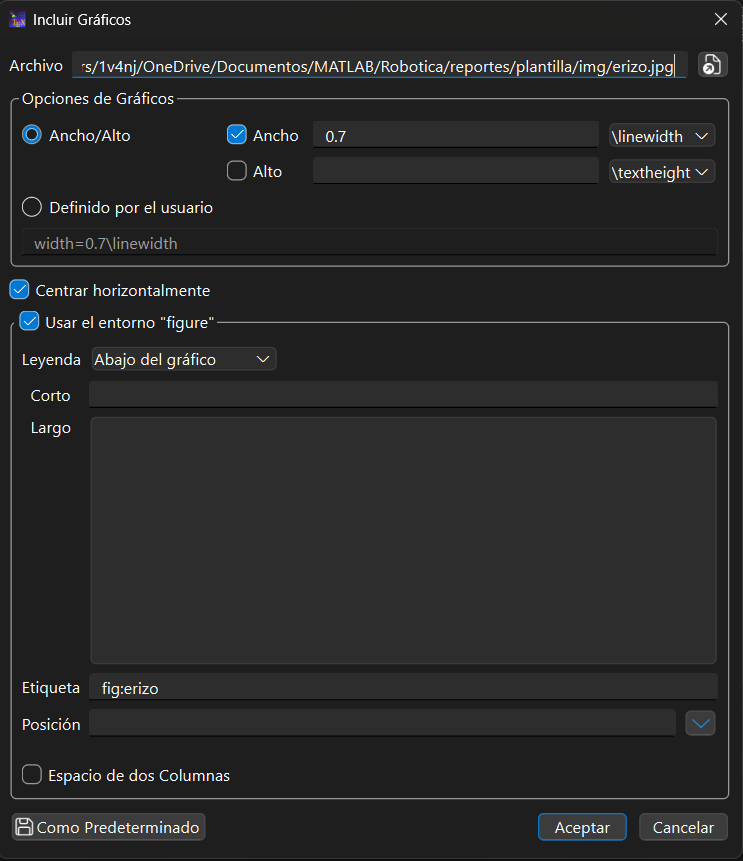
\includegraphics[width=0.7\linewidth]{img/insertarImagen}
	\caption{Opciones al insertar una imagen}
	\label{fig:insertarimagen}
\end{figure}

Algunas opciones clave incluyen:

\begin{itemize}
	\item \textbf{Tamaño de la imagen}: Se puede definir un ancho o alto relativo a la caja de texto o se puede usar un tamaño en pixeles (px), centímetros (cm) o el ancho de la letra M (em).
	\item \textbf{Centrado}: Se puede marcar la opción para que la imagen aparezca centrada automáticamente.
	\item \textbf{Uso del entorno `figure'}: Permite que la imagen tenga una numeración automática y pueda referenciarse en el texto con \texttt{\textbackslash ref\{\}} o \texttt{\textbackslash autoref\{\}}.
	\item \textbf{Posicionamiento (`h`, `t`, `b`, `p`)}: Al presionar la flecha de la derecha, podemos añadir las opciones que determinan la posición de la imagen en el documento, como después del texto o arriba de la página, etc. Si igual vamos a referenciar las figuras, es innecesario que estén exactamente donde fueron mencionadas ya que eso deja muchos espacios en blanco.
	\item \textbf{Leyenda Largo}: permite poner una descripción de la imagen en el lugar que elegimos (debería de estar debajo).
	\item \textbf{Etiqueta}: nos servirá para referenciarla. 
\end{itemize}

Para usar dos imágenes como en \autoref{fig:mascotas}, se utilizó \texttt{subfloat}.
% Dos imágenes de mascotas
\begin{figure}[h]
	\centering
	\subfloat[Perro]{%
		\includegraphics[width=0.4\textwidth]{perro.jpg}%
		\label{fig:perro}
	}
	\hfill
	\subfloat[Gato]{%
		\includegraphics[width=0.4\textwidth]{gato.jpg}%
		\label{fig:gato}
	}
	\caption{Imagen de dos mascotas}
	\label{fig:mascotas}
\end{figure}

%-------------------------------------------
% Bibliografía
%-------------------------------------------
\bibliographystyle{IEEEtran}  % Estilo de bibliografía IEEE
% La bibliografía se tomará del archivo "fuentes.bib"
%\bibliography{fuentes}
	
\end{document}
